\chapter{Hardware Implementierung}



\section{Komponenten}

\begin{itemize}
    \item{Raspberry Pi 4 1 GB}
    \item{COEX Clover 4.2}
\end{itemize}

\section{COEX Clover 4.2}
Bei der für das Projekt verwendete Drohne handelt es sich um eine Coex Clover Drohne in der Version Clover 4.2. Dies ist eine programmierbare Drohne, die besonders für Bildungszwecke eingesetzt wird. Sie ist sowohl für den Einsatz draußen sowie auch in Gebäuden geeignet. \\

\begin{figure}[htpb]
    \centering
    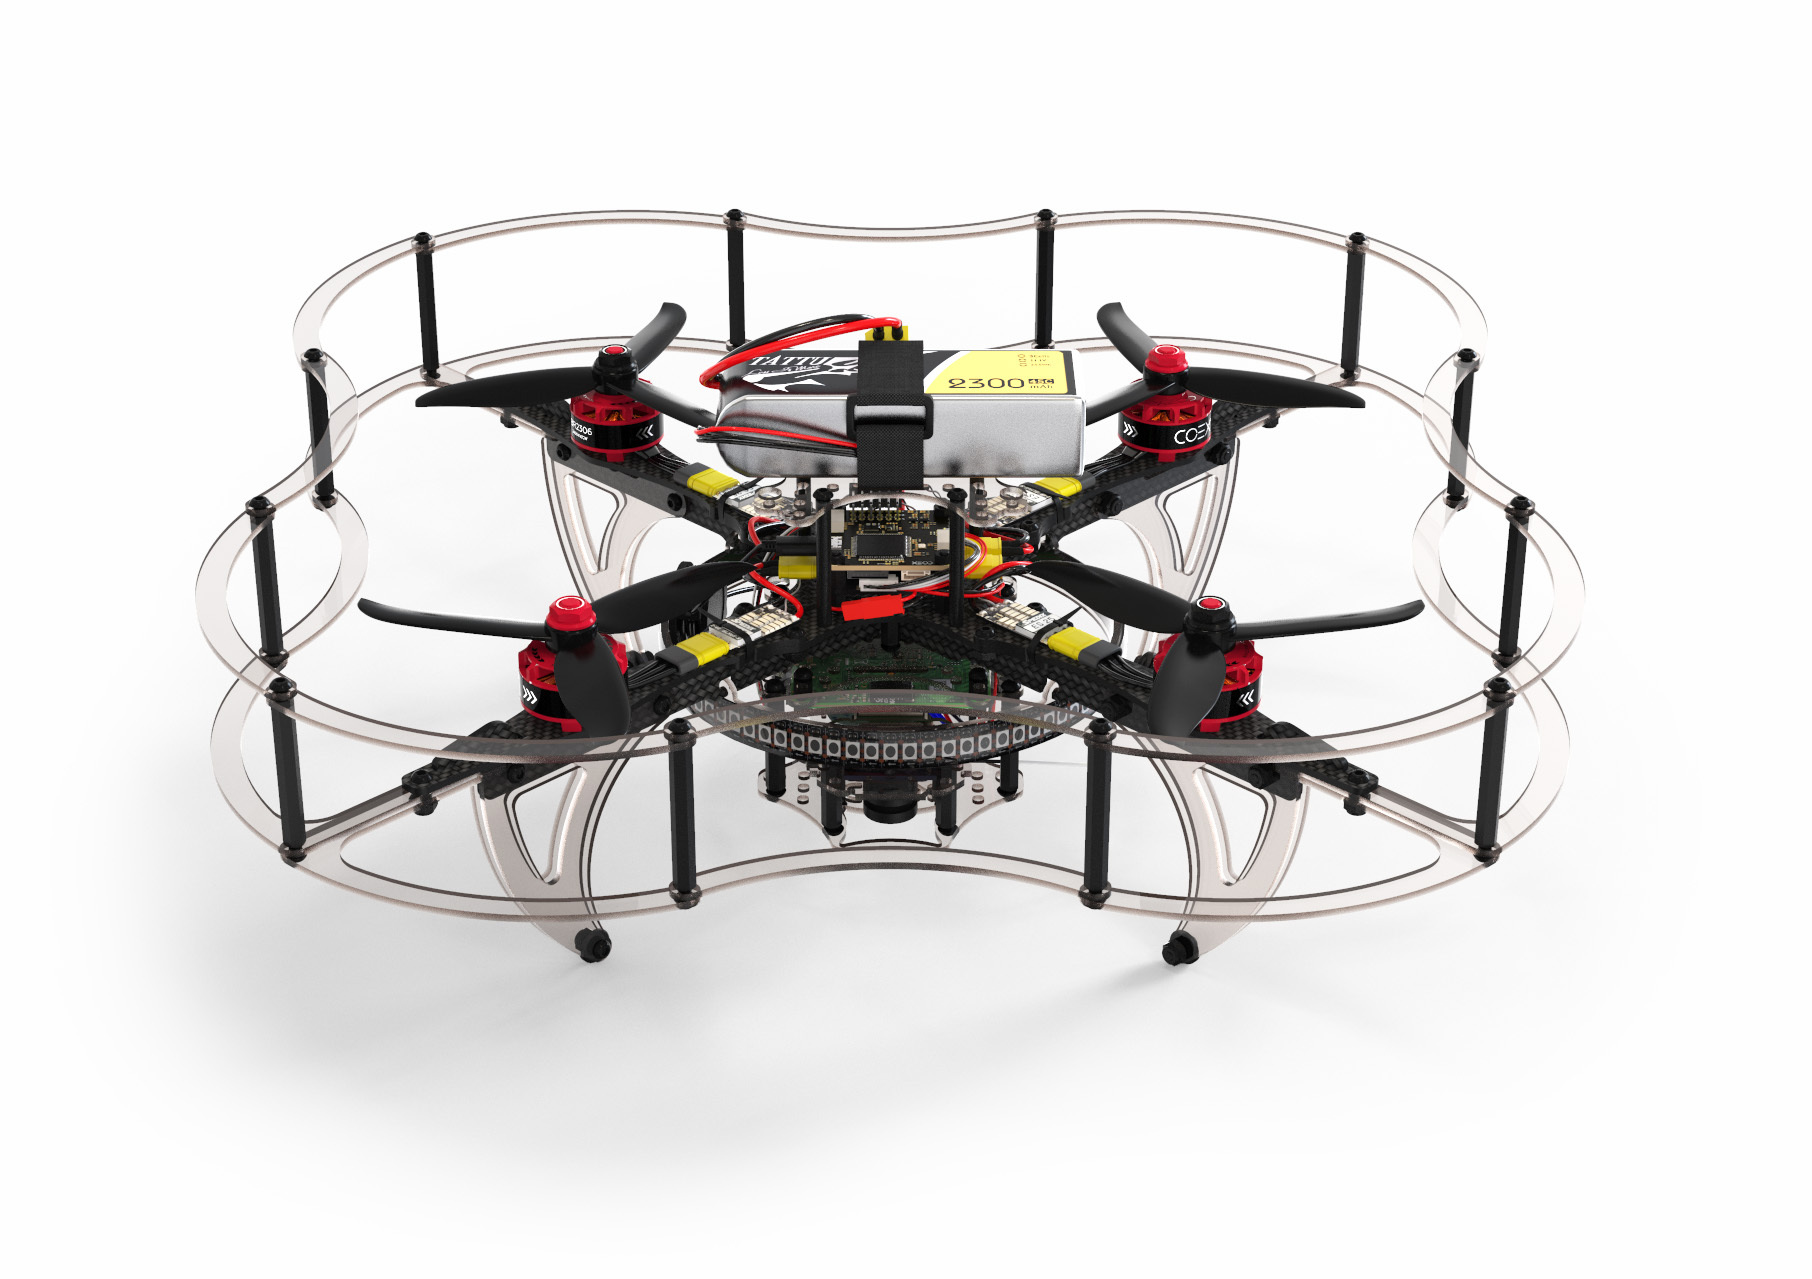
\includegraphics[width=10cm,keepaspectratio,angle=0]{images/coex_clover.jpg}
    \caption[Coex Clover Drohne]{\label{img coex_clover} Coex Clover Drohne \cite{imgcoexclover}}
\end{figure}


Zu Beginn erhält man hierbei einen Bausatz, welcher dann zu einem Quadrokopter zusammengebaut werden kann. Der Vorteil hierbei ist zudem, dass die gesamte Drohne ohne Löten zusammengesetzt werden kann. Zu den einzelnen Bestandteilen der Drohne kommen, noch eine Dokumentation sowie verschiedene Bibliotheken, die es ermöglichen, die Drohne zusammen bauen und fliegen lassen zu können. \\
Durch die Verwendung verschiedener Open-Source Komponenten lässt sich die Drohne programmieren, wodurch ein vielseitiger Einsatzbereich entsteht.\\

\begin{figure}[htpb]
    \centering
    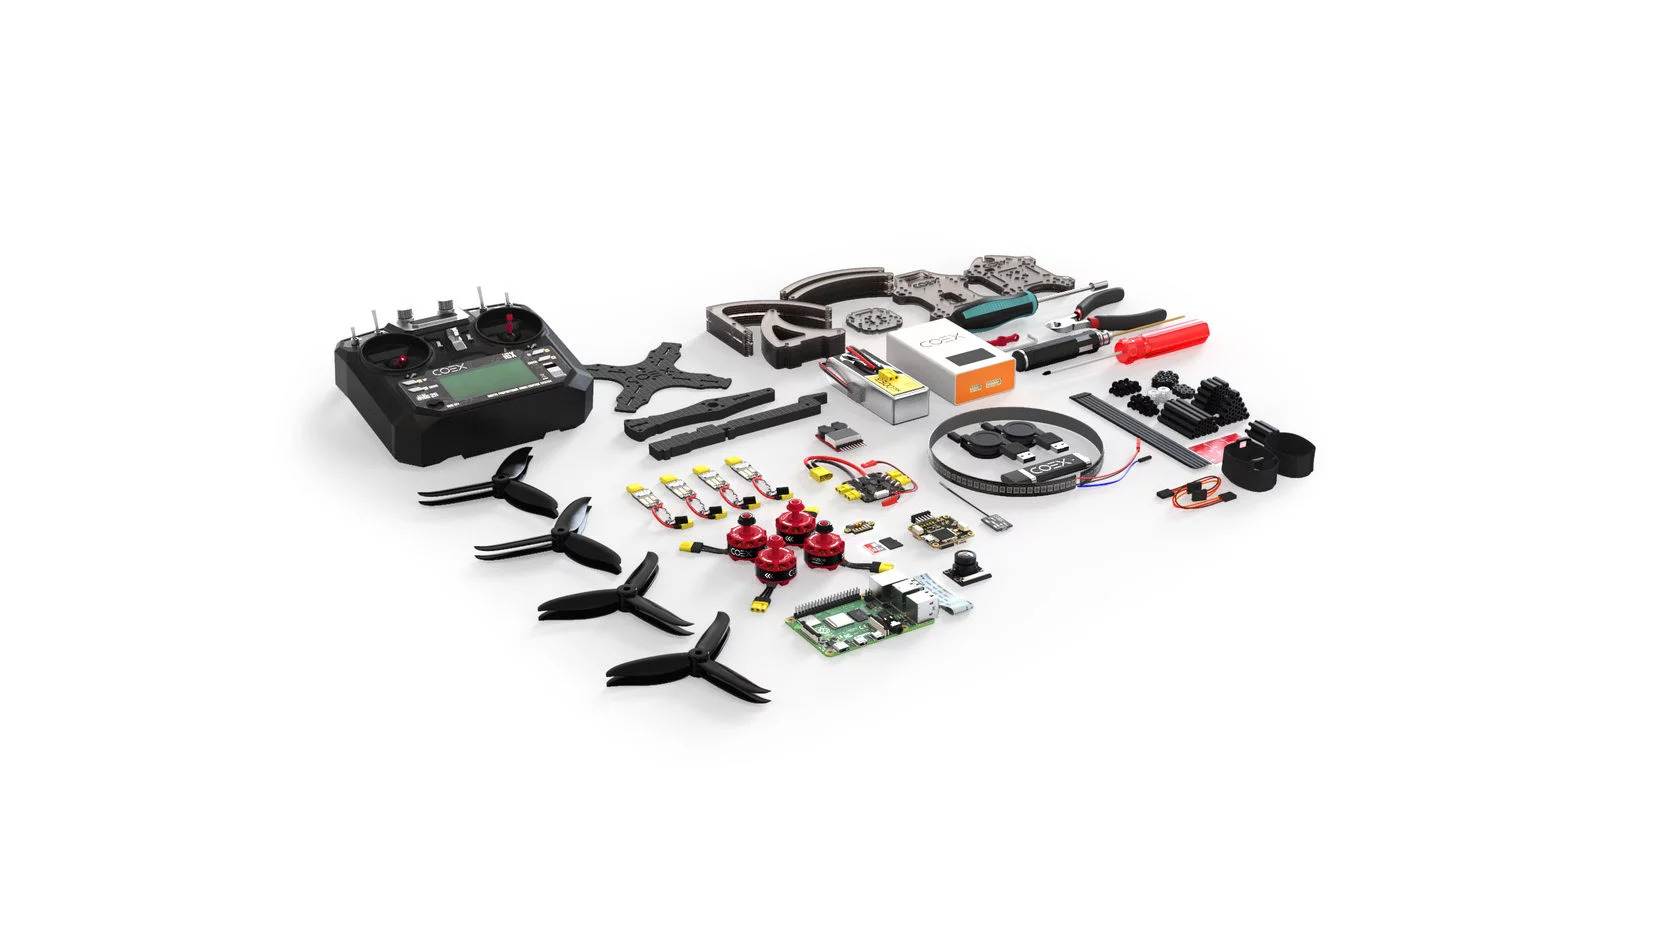
\includegraphics[width=10cm,keepaspectratio,angle=0]{images/coex_clover_kit.jpg}
    \caption[Bausatz Coex Clover Drohne]{\label{img coex_clover_kit} Bausatz Coex Clover Drohne \cite{imgcoexcloverkit}}
\end{figure}

Die Coex Clover Drohne soll laut Herstellerinformationen bis zu 15 Minuten am Stück fliegen können und in dieser Zeit eine Maximalhöhe von 500 Metern bei einer Höchstgeschwindigkeit von bis zu 72 km/h erreichen können \cite[vgl.][]{coex_clover}.\\

Zu den Hauptbestandteilen der Drohne zählen zum einen ein Raspberry Pi 4 sowie der Flightcontroller Coex Pix. Diese bilden die Grundlage zur Programmierung und Steuerung der Coex Clover Drohne und ermöglichen es zudem die Drohne über drahtlos per WLAN zu verbinden. \\
Die Drohne ist ein Quadrokopter und besitzt somit vier Motoren, welche einzeln angesteuert werden können. Sie besitzt zudem eine Vielzahl verschiedener Sensoren, auf welche in Kapitel \ref{sensoren:section} genauer eingegangen wird. Zu diesen zählen unter anderem ein Gyroskop, Magnetometer sowie ein Laseranstandssensor und eine Kamera, die unten an der Drohne angebracht sind.
Zum Schutz befindet sich zudem außen einen Rahmen.
Bei der Drohne war zudem ein 2300 mAh großer Akku dabei, der für vom Hersteller angegebene Flugdauer sorgen soll.
Im Folgenden wird nun auf die wichtigsten Bestandteile der Coex Clover Drohne noch einmal genauer eingegangen:

\subsection{Raspberry Pi 4} \label{raspberry_pi:subsection}

Die Coex Clover Drohne, welche für diese Arbeit genutzt wurde, enthält einen Raspberry Pi 4 Model B mit 1 GB Arbeitsspeicher.\\
Der Raspberry Pi beinhaltet zudem eine austauschbare MicroSD-Karte, auf welche sich in diesem Fall das Raspberry Pi Betriebssysteme befindet. \\

\begin{figure}[htbp]
    \centering
    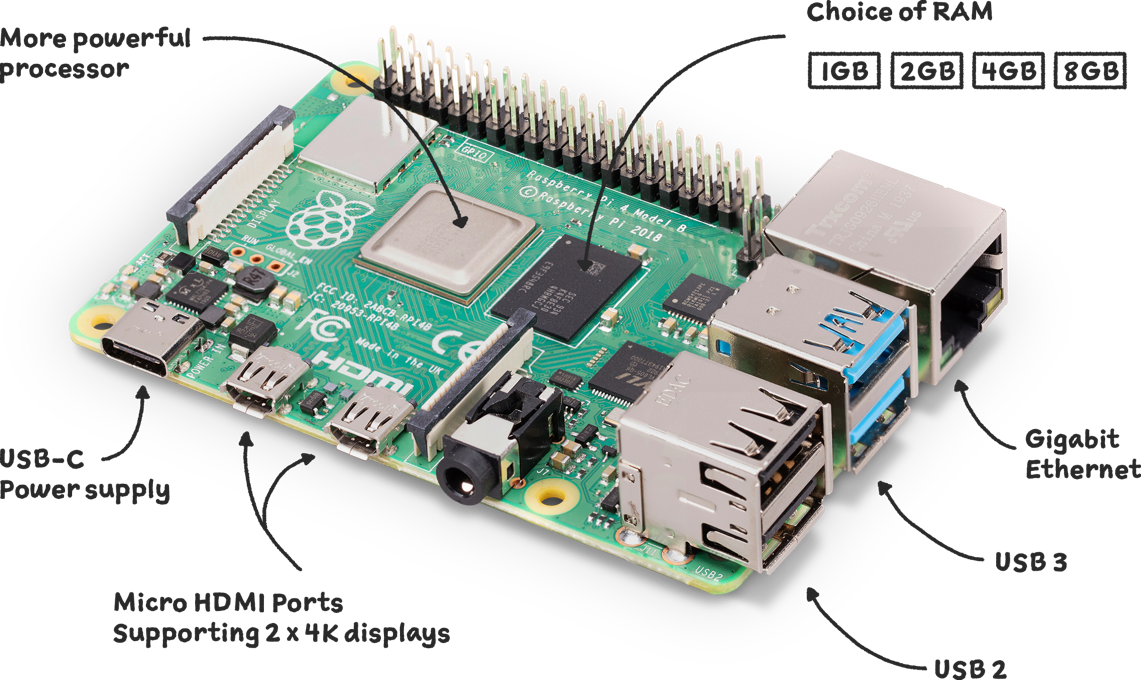
\includegraphics[width=10cm,keepaspectratio,angle=0]{images/raspberry-pi-4-labelled.png}
    \caption[Raspberry Pi 4]{\label{img raspberry_pi} Raspberry Pi 4 \cite{imgraspberrypi}}
\end{figure}

% sets barrier between this subsections so the picture is above the next subsection
\FloatBarrier

\subsection{Coex Pix} \label{coex_pix:subsection}
Der Coex Pix Flight Controller wird für den Betrieb von Drohnen und anderen Fluggeräten verwendet werden. Hierbei basiert dieser auf der PX4 Software. Der Flight Controller einhaltet verschiedene Sensoren, hierzu gehören ein Accelerometer, Gyroskop und ein Magnetometer.

\todo{Benennung FlightController/FlugController/...}

\subsection{Abstandssensor}

\subsection{PX4 FlightController}

\begin{itemize}
    \item{Barometer}
    \item{Gyroskop}
    \item{Accelerometer}
    \item{Magnetometer}
\end{itemize}

\subsection{Kamera}

\section{3D Scanner}

\subsection{Microsoft Hololens}

\section{Azure Kinect DK}

Das Azure Kinect DK ist ein System, das für die Erfassung von Tiefenbildern und 3D-Modellen eingesetzt wird. Das System besteht aus einer RGB-Kamera und einer Tiefenkamera, die in Kombination arbeiten, um präzise räumliche Tiefeninformationen zu erfassen und 3D-Modelle zu generieren.

\subsection{Kamera} \label{kamera:section}
Eine Kamera ist ein Gerät, das in der Lage ist, visuelle Informationen aufzunehmen und zu speichern. Die Funktionsweise einer Kamera basiert auf der Verwendung von optischen Linsen und einem Bildsensor. Das Licht fällt durch die Linse auf den Bildsensor, der das Licht in elektronische Signale umwandelt, die dann von einem Prozessor verarbeitet und in ein digitales Bild umgewandelt werden. Der Prozessor kann auch Funktionen wie Fokussierung, Belichtung und Weißabgleich steuern. Die resultierenden digitalen Bilder können dann gespeichert oder übertragen werden. 

Das Azure Kinect \ac{DK} verwendet 2 Kameras, wie in Auflistung \ref{azure-kamera}

\begin{description}

    \label{azure-kamera}
    \item[RGB Kamera] Die RGB-Kamera des Azure Kinect DK ist eine hochauflösende Farbkamera, die auf einem 1/2.5" CMOS-Sensor basiert. Die Kamera hat eine Auflösung von 3840 x 2160 Pixeln (4K) und verfügt über einen Rolling-Shutter, der die Bildaufnahme zeilenweise abarbeitet, um Bewegungsunschärfe zu reduzieren. Das System ist in der Lage, Farbinformationen und Texturdaten zu erfassen, die für die Erstellung von 3D-Modellen genutzt werden können.
    \item[Depth Kamera] Die Tiefenkamera des Azure Kinect \ac{DK} nutzt einen Time-of-Flight-Sensor, um Tiefenbilder zu erfassen. Die Kamera sendet Infrarot-Licht aus, das vom Objekt reflektiert und von der Kamera empfangen wird. Die Zeit, die das Licht braucht, um zum Objekt und zurück zur Kamera zu gelangen, wird gemessen und zur Berechnung der Entfernung genutzt. Die Auflösung der Tiefenkamera beträgt 1024 x 1024 Pixel, was für eine präzise Erfassung der Tiefeninformationen ausreichend ist. Die Tiefenkamera untersützt verschiedene Modi. Folgende Modi werden unterstützt.

\begin{itemize}
        \item NFOV\_UNBINNED (NFOV): Normaler Sichtbereich, unbinär (ungebündelt) und unverzerrt. Eignet sich für die meisten Anwendungen und liefert eine präzise Tiefenkarte mit hoher räumlicher Auflösung.
        \item NFOV\_BINNED (NFOV): Normaler Sichtbereich, binär (gebündelt) und unverzerrt. Bietet eine höhere Bildrate und eignet sich für Anwendungen, die keine hohe räumliche Auflösung benötigen, wie z.B. Körperverfolgung oder Objekterkennung.
        \item WFOV\_UNBINNED (WFOV): Weitwinkel-Sichtbereich, unbinär und unverzerrt. Bietet eine größere Abdeckung des Sichtbereichs und ist ideal für Anwendungen wie z.B. Umgebungserkennung oder Indoor-Kartierung.
        \item WFOV\_BINNED (WFOV): Weitwinkel-Sichtbereich, binär und unverzerrt. Bietet eine höhere Bildrate und ist nützlich für Anwendungen wie z.B. Körperverfolgung oder Objekterkennung in einem breiteren Sichtbereich.
        \item PASSIVE\_IR (IR): Infrarot-Sichtbereich, binär und unverzerrt. Eignet sich für Anwendungen, bei denen Lichtbedingungen schlecht sind oder Infrarot-Signale genutzt werden, wie z.B. bei der Erfassung von Gesten.
    \end{itemize}
\end{description}

    

    Durch die Kombination von RGB- und Tiefenkamera ist das Azure Kinect \ac{DK} in der Lage, präzise räumliche Tiefeninformationen zu erfassen und 3D-Modelle zu generieren. Das System kann in einer Vielzahl von Anwendungen eingesetzt werden, wie zum Beispiel in der Robotik, virtuellen Realität und Augmented Reality. Es kann auch für die Erfassung von Bewegungen und Gesten genutzt werden, was in der Computergrafik und im Maschinenlernen von Vorteil ist.


    Zusätzlich zur RGB- und Tiefenkamera verfügt das Azure Kinect \ac{DK} auch über eine integrierte Inertial Measurement Unit (\ac{IMU}). Die \ac{IMU} besteht aus einem Beschleunigungsmesser und einem Gyroskop, die Bewegungsdaten erfassen und zur Bestimmung der Orientierung und Position des Geräts im Raum genutzt werden können. Die \ac{IMU} kann auch zur Kompensation von Bewegungsunschärfe und zur Stabilisierung von 3D-Modellen genutzt werden.

\subsection{\acl{IMU}}

Das Azure DK (Development Kit) enthält eine integrierte IMU (Inertial Measurement Unit), die aus einem 3-Achsen-Beschleunigungsmesser und einem 3-Achsen-Gyroskop besteht. Die IMU erfasst die Beschleunigung und Rotation des Geräts und liefert entsprechende Daten, die für die Navigation und Stabilisierung verwendet werden können.

Die \ac{IMU} im Azure Kinect \ac{DK} ist speziell darauf ausgelegt, zusammen mit den Kameras des Systems zu arbeiten. Sie ist in der Lage, genaue Daten in Echtzeit zu liefern und kann zur Verbesserung der räumlichen Genauigkeit der Tiefenbilder beitragen. Die IMU kann auch in Kombination mit anderen Sensoren und Systemen genutzt werden, um die Bewegung und Position von Geräten und Robotern in Echtzeit zu verfolgen.
Im Kapitel \todo{referenz} wird auf die Zusammenarbeit von Kamera und IMU eingegangen.

Insgesamt ermöglicht die Integration einer \ac{IMU} dem Azure Kinect \ac{DK} eine noch präzisere und zuverlässigere Erfassung von Tiefeninformationen und Bewegungsdaten. Dies macht das System zu einem leistungsfähigen Werkzeug für eine Vielzahl von Anwendungen in der Robotik, virtuellen Realität, Augmented Reality und anderen Bereichen, in denen eine genaue räumliche Erfassung erforderlich ist.

    \todo{Quellen}